\documentclass[]{report}   % list options between brackets
\usepackage[textwidth=15cm, textheight=20cm]{geometry}              % list packages between braces
\usepackage{graphicx}
\usepackage{float}
\usepackage{cite}
\usepackage{url}
\renewcommand\thesection{\arabic{section}}

\begin{document}

\title{QR Codes for Security and Authentication}
\author{Andy Hansen\\\\
Supervised by David Eyers} 
\date{July 17, 2014} 
\maketitle
\tableofcontents

\section{Introduction}
QR codes have been around since 1997, but have been used for little more than putting website URLs into a physically scannable form. The aim of my project is to see if there are interesting ways we can use QR codes as a way of authenticating a user and setting up a secure channel of communication between a user and the services they wish to access. We plan to use Android smartphones as a means of generating and displaying the user's credentials in QR code form, so that they may be scanned by the service and grant them access without the user having to enter their username and password directly where it could be compromised. The user's details will sometimes be combined with context information proving that the intended user is the one scanning the QR code or codes.

In this report I am going to give an overview of my infrastructure, explain what my system is currently capable of, give the advantages of technologies I have picked, and talk about what I will be doing in the future.

\section{Background}    
\subsection{Kerberos}   
Kerberos \cite{Kerb} is a computer network authentication protocol which allow nodes to prove their identity to one another in a secure way. It uses ‘tickets’ as its mechanism to prove identity, a valid user will have a ticket to give to the service they wish to access. Kerberos allows both the user and the server to identify each other. When a user logs into the Kerberos key distribution center (KDC) they are given a ticket granting ticket (TGT). The TGT is presented by the user when they wish to access a restricted service, if the service accepts the user's TGT they will be given a ticket specific to the service when they can then use to access it securely. Kerberos is single sign on meaning that once a user gets their TGT, they will not need to login again until it expires.

 
\subsection{QR Codes}  
A QR, or Quick Response code \cite{QR} is a specially formatted image which is designed to be quickly read by a camera. QR codes come in a variety of versions, a version refers to how many rows and columns there are in the code, a high version code is going to be able to store more information, but will also be harder to read. QR codes store data using one of four different modes: numeric only, alphanumeric, byte/binary (ISO8859-1), and kanji. The mode affects how many characters can be stored within the QR code e.g. A numeric only code will be able to store more than the alphanumeric code.

\section{Considerations} 
\subsection{Kerberos Ticket Expiry Times} 
I need to consider the ideal ticket expiry time. The attackers effective time window needs to be reduced as much as possible without inconveniencing the user. Since the tickets are held on the user’s phone, I want to make the tickets expire faster but allow the user to easily get more tickets once they do. I will need to do some research to find the ideal amount of time for a ticket to stay alive so that a user does not feel inconvenience, will still making it hard for an attacker to use the ticket for very long after it has been intercepted. 

\subsection{QR Code Versions}
When there are many tickets to encode it will take multiple QR codes to store all of the information. It is important that users do not feel inconvenienced by this, so the right QR code version needs to be used which is fast to scan and uses minimal codes. Picking the right QR code version is quite difficult because there are many factors to consider: screen size, pixel density, and camera quality when scanning the QR codes. A ticket can easily fit into a version 40 QR code, but it is very hard for a scanner to read it, especially when the QR code is displayed on a screen with low resolution. Tickets around version 20 can be reliably and quickly scanned, but this does not mean they are the ideal. I will be performing some tests in semester 2 to find the ideal code version so I can use minimal QR codes, and still have them easy to scan.

\begin{figure}[H]
\centering
%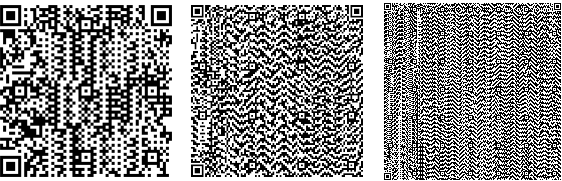
\includegraphics[width=9cm]{QRCodes.png}
\caption{QR code versions 10, 20, and 40 respectively.}
\end{figure}

\section{My Progress}
\subsection{Infrastructure} 
I will give a brief overview of how my infrasture is set up and explain the advantages of the technologies I have chosen. My current infrastructure involves two servers that are both running Ubuntu 14.04. The first server is used as the Kerberos key distribution center (KDC) running version 5 and a domain name server that uses Bind version 9 \cite{Bind}, the second server hosts an Apache web server which can be only be accessed with a valid Kerberos ticket from the KDC server. At the moment the Apache server is playing the role of any possible future Kerberos enabled service. It is a good service to use when testing because there is instant visual feedback when it is working. A use case that results in me being able to access the Apache server could be replaced with any other service such as SSH or access to my account from the login GUI.

I am using Kerberos because it is runs on all popular operating systems and has built in support in a lot of existing services such as Apache, SSH, and Samba. This means that when a service is configured to connect with the user's KDC, they can use their TGT to access restricted web pages, ssh into protected machines, and access specific folders. I am using Kerberos version 5 because it is the most recent and has resolved some security concerns that were present in version 4 \cite{KerbUpdate}. Kerberos is also useful because all tickets have an expiry time. This is important in my system because if a man in the middle attack is performed, then the attacker can only abuse the until it expires. Kerberos is single sign on which is useful in our QR code based system because the user does not have to enter their username and password for each individual service they are trying to access. It is a protocol that is supported on all major operating systems and is well tested. If I was to try and design an authentication protocol myself it would require me to do all of the integration and testing which would take a long time without providing very much benefit.

In my project QR codes are going to be used as a primary communication channel between the user and their services. QR codes are a good option because they are easy to use, and hard to perform a man in the middle attack on. The malicious user would have to get a copy of all the user's QR codes before they could use them themselves.

Unfortunately QR codes do not have support direct binary encoding, this means that Kerberos tickets (which are stored in binary) need to be converted to an alphanumeric format before being encoded. I am currently converting the tickets to hex but in the future I will convert them to base64 because it makes more use of the alphanumeric character set, allowing QR code sizes to be reduced further.

\subsubsection{Proof of Concept} 
I am going to give a run through of my basic use case to show how a user’s ticket can be transferred from one machine to another using QR codes \cite{YouTubeDemo}. Though basic, it proves that it is possible to for a program to be implemented using a phone which can store Kerberos tickets as QR codes, and for a scanned QR code to be put into the ticket cache as a valid Kerberos ticket. My proof of concept operates as outlined here:

\begin{itemize}
	\item Both computer A and B have no Kerberos tickets, and therefore are unable to access the Apache server.
	\item Computer A runs kinit which is a command line program used to authenticate a user to the Kerberos KDC and get their TGT. They enter their details and are given their TGT. They can then use this ticket to negotiate a ticket for the Apache server, granting them access to its resources.
	\item Computer A then runs the QR code creating program. The program takes the TGT from the ticket cache (the location Kerberos tickets are stored) and converts it to hex, it then takes the hex and splits it into small sections. Each of those sections are then encoded into a QR code with a number used to identify the order of the QR codes so they can be reassembled. 
	\item Computer B, which is running the QR code scanning software, scans each of the QR codes created by Computer A. When all the codes are decoded they are reassembled using the ordering numbers from before, converted back to binary, and then added to the Kerberos ticket cache. Computer B is now able to use the TGT just as Computer A could before to negotiate a ticket to access the Apache server.
	\item The tickets from computer A have now been transferred solely using QR codes as the primary means of communication.
\end{itemize}

In the future this use case would replace computer A with an Android smartphone, they would be able to scan their code on any computer running my QR code scanning program to get authenticate themselves and gain access to the services they are allowed to, such as the Apache server above.


\subsubsection{Difference From Aims and Objectives} 
I originally planned for there to be more interaction with the phones sensors as a way of confirming the phone is in the same location as the scanned QR code. Instead of this I am now having all of the information coming from the QR codes. This puts less requirements on the sensors for anywhere my QR code scanning software is running, and makes the average user interaction faster because all they have to do is scan their QR code. GPS information is also not available indoors which limits its usefulness since all use cases will be performed indoors. Instead we are going to allow users to prove their location by scanning room specific QR codes which I feel is a good trade off between security and ease of use.


\section{Related Work}
\subsection {Web Authentication Using A Mobile Phone}
This is a method of authentication using a mobile phone, but rather than using a QR code to authenticate the user it puts a proxy between the user and an untrusted computer they need to use \cite{MobileRelated}. The proxy server stores the usernames and passwords. A text message is used to authenticate the user's session to the proxy, and the proxy acquires the login sessions for the user so they do not have to enter usernames and passwords on the suspicious computer.

My solution takes a different approach to this one, theirs can run on any computer because they just need to connect to their secure proxy. I sacrifice the ability to work anywhere for allowing more uses than just the web, and users of my program can transfer their permissions from one computer to another without having to enter their username and password again. 

\subsection{QR Code Based Door Access}
This project uses QR codes to open doors \cite{QRRelated}. The QR code does not expire which is dangerous, but it seems the main purpose of the project is for convenience over security. The idea behind their project is that a user can be emailed their access codes and seem intended to replace key cards. The problem with this method is that replay attacks could be set up to copy a user's QR code and give it to the attacker.

My implementation differs from this because rather than storing an access key, the QR codes in my system store the TGT which could be used to get the user a login session at a computer as well as room access. Their system sends QR codes via email. If someone was able to perform a man in the middle on their mailserver they could gain access to every QR code emailed out.


\section{Future Work}
A big part of my project is coming up with ways the QR codes can be used and then implementing them. We have come up with some potential use cases, and this semester I am working out the specifics involved in the use cases and implementing them. I’m going to go through some of my considered use cases and work out any of the details. I also need to implement the Android application so that these use cases can be carried out in a portable manner.

\subsection{Android Application}
In my proof of concept I have shown what my system is capable of doing, but in the future I want the user to be able to start the interaction with an Android smartphone. The reason Android is the target platform is because MIT Kerberos has been ported to it \cite{KerbDroid}. There is also an open source application I can use as a reference on how to build my own Kerberos application \cite{KerbApp}. My use cases should have low processing requirements so even modest processors will be able to run my application. Smartphones also come with cameras, Wi-Fi, and displays built in. This means that my use cases can include the user connecting to the internet, scanning QR codes with their camera, or displaying QR codes on their screen without fear that user will not have the hardware to perform these actions.

\subsection{Collaboration On A LAN}
In the future I want to be able to use the Android application as a means of establishing trust between a group collaborating on a LAN. The master user could create a QR code which can be scanned by all the other users. They use the information in this QR code to set up a trust relationship between their own KDC and the KDC of the LAN they are collaborating on. Once this trust is set up, each of the users can use their own Kerberos account to access services on the network they are collaborating on without having to get their own account for the LAN. It also means that the owner of the LAN’s KDC can discontinue the trust with any KDCs of users leaving the LAN. With this use case there is potential for a user to cause damage to any services they are give access rights to, but the user who caused the damage will be known because they must use their own account, and the trust can be broken with them at anytime, stopping their access.

\subsection{Transferring A Login Session}
I also want to allow a user to take their login session elsewhere using their phone. The idea is that if a user has already logged in then they should be able to take that session with them on their phone and continue it on the same network without entering their details again. Upon logout the user has the option to receive QR codes for their phone which contains their TGT. They can scan the QR codes from their phone at any other computer on the network running my QR code scanning program and it will place their TGT into the ticket cache and log them in without them having to enter their details. For this use case to operate correctly I need to be able have my program as part of the login GUI. Possible threats with this use case are that a user could be out of the room and have a malicious user come and “steal” their login session, this is something I will need to consider when making the program.

\begin{thebibliography}{9}
\bibitem{Bind} Douglas B. Terry, Mark Painter, David W. Riggle Songnian Zhou, The Berkeley Internet Name Domain Server, 1984.   
\bibitem{Kerb} B. Clifford Neuman, Theodore Ts'o, Kerberos: An Authentication Service for Computer Networks, 1994. 
\bibitem{QR} Needed.
\bibitem{KerbDroid} krb5-anonsvn, \url{https://github.com/cconlon/krb5-anonsvn}, 2014.
\bibitem{KerbApp} kerberos-android-ndk, \url{https://github.com/cconlon/kerberos-android-ndk}, 2014.
\bibitem{KerbUpdate} Kerberos Version 4 End of Life Announcement, \url{http://web.mit.edu/kerberos/krb4-end-of-life.html}, 2014.
\bibitem{MobileRelated} Secure Web Authentication with Mobile Phones, \url{http://homepages.mcs.vuw.ac.nz/~ian/shared/papers/secureweb.pdf}, 2014.
\bibitem{QRRelated} LibeTech QR Code Door Lock, \url{http://www.jeremyblum.com/portfolio/libetech/}, 2014.
\bibitem{YouTubeDemo} QR Code Proof of Concept, \url{https://www.youtube.com/watch?v=v8ZZWC-jXeM\&list=UU3CfgH3Wtm0TTpxq0I92XFw}, 2014.
\end{thebibliography}

\end{document}